%%%%%%%%%%%%%%%%%%%%%%%%%%%%%%%%%%%%%%%%%%%%%%%%%%%%%%%%%%%%%%%
%
% Welcome to Overleaf --- just edit your LaTeX on the left,
% and we'll compile it for you on the right. If you open the
% 'Share' menu, you can invite other users to edit at the same
% time. See www.overleaf.com/learn for more info. Enjoy!
%
%%%%%%%%%%%%%%%%%%%%%%%%%%%%%%%%%%%%%%%%%%%%%%%%%%%%%%%%%%%%%%%
% Author: Izaak Neutelings (December 2020)
% http://hyperphysics.phy-astr.gsu.edu/hbase/Waves/standw.html
\documentclass[border=3pt,tikz]{standalone}
\usepackage{amsmath}
\usepackage{etoolbox} % ifthen
\usepackage{tikz}
\usetikzlibrary{arrows.meta} % for arrow size
\tikzset{>=latex} % for LaTeX arrow head

\colorlet{myred}{red!65!black}
\colorlet{xcol}{blue!70!black}
\colorlet{vcol}{green!60!black}
\colorlet{Pcol}{orange!80!black}
\colorlet{dense air}{Pcol!70!red!60}
\colorlet{thin air}{brown!10}
\tikzstyle{vvec}=[->,vcol,very thick,line cap=round]
\tikzstyle{force}=[->,myred,thick,line cap=round]
\tikzstyle{wood}=[very thick,brown!70!black]
\tikzstyle{piston}=[blue!50!black,top color=blue!30,bottom color=blue!50,middle color=blue!20,shading angle=0]
\tikzstyle{walldark}=[blue!20!black,top color=black!10!white!90!blue,bottom color=black!20!white!90!blue,shading angle=-30]
\tikzstyle{wall}=[blue!20!black,top color=black!5!white!90!blue,bottom color=black!10!white!85!blue,shading angle=30]
\def\tick#1#2{\draw[thick] (#1) ++ (#2:0.1) --++ (#2-180:0.2)}
\tikzstyle{myarr}=[xcol!50,-{Latex[length=3,width=2]}]

\begin{document}

%% AIR PARTICLE DENSITY - test
% \begin{tikzpicture}
%     \def\lam{2.0} % wavelength
%     \def\N{1000}
%     \fill[left color=white,right color=white,middle color=blue!80!black!30]
%     (0,0) rectangle (\lam/2,1);
%     \fill[left color=white,right color=white,middle color=blue!80!black!30]
%     (\lam/2,0) rectangle (\lam,1);
%     \draw (0,0) rectangle++ (\lam,1);
%     \foreach \i in {1,...,\N}{
%             \fill[blue!40!black] ({acos(-rand)*\lam/360},{(1+rand)/2}) circle(0.008);
%             \fill[blue!40!black] ({\lam/2+acos(-rand)*\lam/360},{(1+rand)/2}) circle(0.008);
%         }
% \end{tikzpicture}


%% AIR PARTICLE DENSITY - visual approximation - test
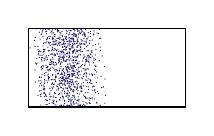
\begin{tikzpicture}
    \def\lam{2.0} % wavelength
    \def\N{500}
    % \fill[left color=white,right color=white,middle color=blue!80!black!30]
    % (0,0) rectangle (\lam/2,1);
    % \fill[left color=white,right color=white,middle color=blue!80!black!30]
    % (\lam/2,0) rectangle (\lam,1);
    \draw (0,0) rectangle++ (\lam,1);
    \foreach \i in {1,...,\N}{
            \fill[blue!40!black] ({\lam/2*sqrt((rand+1)/8)},{(1+rand)/2}) circle(0.008);
            \fill[blue!40!black] ({\lam/2-\lam/4*sqrt((1-rand)/2)},{(1+rand)/2}) circle(0.008);
            % \fill[blue!40!black] ({\lam/2+\lam/2*sqrt((rand+1)/8)},{(1+rand)/2}) circle(0.008);
            % \fill[blue!40!black] ({\lam-\lam/4*sqrt((1-rand)/2)},{(1+rand)/2}) circle(0.008);
        }
\end{tikzpicture}

% TRAVELLING WAVE
% \begin{tikzpicture}
%     \def\ymax{0.85}    % y maximum
%     \def\xmax{5.5}     % x maximum
%     \def\A{0.80*\ymax} % amplitude
%     \def\D{1.20*\ymax} % pipe diameter
%     \def\lam{2.0}      % wavelength
%     \def\L{0.97*\xmax} % length
%     \def\s{2.45*\ymax} % shift
%     \def\nwaves{3}     % number of waves
%     \def\N{1200}       % number of points
%     %\def\N{100}        % number of points

%     % DISPLACEMENT
%     \foreach \i [evaluate={\x=(\i-0.5)*2*\lam/4;}] in {1,...,5}{
%             \ifodd\i \def\sgn{1} \else \def\sgn{-1} \fi % y position
%             \draw[myarr] (\x,\sgn*0.15*\A) --++ (0,\sgn*0.65*\A);
%             \draw[blue!20!black!60,very thin,dashed] (\x+\lam/4,\ymax) --++ (0,-2.1*\s);
%         }
%     \draw[->,thick] (0,-\ymax) -- (0,0.1+\ymax) node[below=2,left] {$s$};
%     \draw[->,thick] (-0.2*\ymax,0) -- (0.2+\xmax,0) node[below] {$x$};
%     \draw[xcol,very thick,samples=100,smooth,variable=\x,domain=0:\L]
%     plot(\x,{\A*sin(360/\lam*\x)});
%     %\draw[xcol,dashed,samples=100,smooth,variable=\x,domain=0:\L]
%     %  plot(\x,{-\A*sin(360/\lam*\x)});
%     \draw[vvec] (1.45*\lam,0.70*\A) --++ (0.3*\lam,0) node[right=-2] {$v$};

%     % PRESSURE
%     \begin{scope}[shift={(0,-\s)}]
%         \draw[->,thick] (0,-\ymax) -- (0,0.1+\ymax) node[below=2,left] {$\Delta P$};
%         \draw[->,thick] (-0.2*\ymax,0) -- (0.2+\xmax,0) node[below] {$x$};
%         \draw[Pcol,very thick,samples=100,smooth,variable=\x,domain=0:\L]
%         plot(\x,{\A*sin(360/\lam*\x-90)});
%         %\draw[Pcol,dashed,samples=100,smooth,variable=\x,domain=0:\L]
%         %  plot(\x,{-\A*sin(360/\lam*\x-90)});
%         \draw[vvec] (1.70*\lam,0.70*\A) --++ (0.3*\lam,0) node[right=-2] {$v$};
%     \end{scope}

%     % TUBE
%     \begin{scope}[shift={(0,-2.1*\s)}]
%         \fill[thin air] (0,0) rectangle++ (\L,\D);
%         \foreach \i [evaluate={\x=(\i-1)*\lam;\cond=\x+0.75*\lam<\L ? 1 : 0;}] in {1,...,\nwaves}{
%                 \message{^^JWave \i}
%                 \draw[myarr] (\x+0.25*\lam,1.1*\D) --++ ( 0.21*\lam,0);
%                 \ifnum\cond=1
%                     \draw[myarr] (\x+0.75*\lam,1.1*\D) --++ (-0.21*\lam,0);
%                 \fi
%                 \begin{scope}
%                     \clip (0,0) rectangle (\L,\D);
%                     \path[left color=thin air,right color=thin air,middle color=dense air]
%                     (\x,0) rectangle (\x+\lam,\D);
%                     \foreach \i in {1,...,\N}{
%                             \fill[blue!40!black] ({\x+acos(-rand)*\lam/180},{\D*(1+rand)/2}) circle(0.01);
%                         }
%                 \end{scope}
%             }
%         \draw[wood,line cap=round] (\L,\D) -| (0,0) -- (\L,0);
%         \draw[vvec] (0.97*\L,0.50*\D) --++ (0.3*\lam,0) node[right=-2] {$v$};
%     \end{scope}

% \end{tikzpicture}


% PISTON
% \begin{tikzpicture}
%   \def\Ry{0.7}
%   \def\Rx{0.16*\Ry}
%   \def\ry{0.14}
%   \def\rx{0.16*\ry}
%   \def\w{0.08} % wall thickness
%   \def\x{0.18} % piston position
%   \def\L{4.5}  % container length
%   \def\l{1.4}  % piston length
%   \def\v{0.7}  % piston length
%   \def\xu{0.16*\L} % distance with u
%   \def\xv{0.52*\L} % distance with v

%   % WIDTH
%   \draw[->] (\x,-1.22*\Ry) --++ (\xu,0) node[pos=0.4,below=-2] {$u\Delta t$};
%   \draw[->] (\x, 1.22*\Ry) --++ (\xv,0) node[midway,above=-2,fill=white,inner sep=1] {$v\Delta t$};

%   % WALL
%   \draw[wall]
%     (0,\Ry) arc (90:-90:{\Rx} and {\Ry}) --++ (\L,0) arc (-90:90:{\Rx} and {\Ry}) -- cycle;
%   %\draw[walldark] (0,0) ellipse ({\Rx} and \Ry);

%   % SHELL
%   %\draw[piston] % piston steele
%   %  (\x-\l,\ry) arc (90:270:{\rx} and {\ry}) -|++ (\l,2*\ry) -- cycle;
%   %\draw[wall]     (0,0) ellipse ({\Rx} and \Ry);
%   \draw[walldark] (0,\Ry) rectangle++ (\L,\w);
%   \draw[walldark] (0,-\Ry) rectangle++ (\L,-\w);
%   \draw[walldark]
%     (\L,\Ry+\w) arc (90:-90:{\Rx+0.7*\w} and {\Ry+\w}) --++ (0,\w) arc (-90:90:{\Rx} and {\Ry}) -- cycle;

%   % PISTON
%   \draw[piston] % piston steele
%     (\x-\l,\ry) arc (90:270:{\rx} and {\ry}) -|++ (\l,2*\ry) -- cycle;
%   \draw[walldark]
%     (\x,\Ry) arc (90:270:{\Rx} and {\Ry}) --++ (-2*\w,0) arc (-90:-270:{\Rx} and {\Ry}) -- cycle;
%   \draw[piston] (\x,0) ellipse ({\Rx} and \Ry);
%   %\draw[walldark] (\x+\l,0) ellipse ({\rx} and \ry);

%   % BOTTOM
%   %\draw[walldark]
%   %  (0,\Ry) arc (90:270:{\Rx} and {\Ry}) --++ (0,-\w) arc (-90:-270:{\Rx+\w} and {\Ry+\w}) -- cycle;

%   % LABELS
%   \draw[dashed]
%     (\x+\xu,0) ellipse({\Rx} and {\Ry})
%     (\x+\xv,0) ellipse({\Rx} and {\Ry});
%   \draw[force] (\x-0.9*\l,1.7*\ry) --++ (0.6*\l,0)
%     node[midway,above=-1] {$F$};
%   %\draw[<-,thick,blue!60!black] (\x,0.7*\Ry) to[in=-30] (\x,1.2*\Ry)
%   %  node[below=3,above left] {$A$};
%   \draw[very thin,blue!60!black] (\x+0.5*\Rx,-0.35*\Ry) to[out=-20,in=120]++ (1.1*\Rx,-0.16*\Ry)
%     node[below=0,below right=-4] {$A$};

% \end{tikzpicture}


\end{document}